
\documentclass{article}

% if you need to pass options to natbib, use, e.g.:
%     \PassOptionsToPackage{numbers, compress}{natbib}
% before loading neurips_2018

% ready for submission
% \usepackage{neurips_2018}

% to compile a preprint version, e.g., for submission to arXiv, add add the
% [preprint] option:
\usepackage[preprint]{neurips_2019}

% to compile a camera-ready version, add the [final] option, e.g.:
     % \usepackage[final]{neurips_2019}

% to avoid loading the natbib package, add option nonatbib:
%     \usepackage[nonatbib]{neurips_2018}

\usepackage[utf8]{inputenc} % allow utf-8 input
\usepackage[T1]{fontenc}    % use 8-bit T1 fonts
\usepackage{hyperref}       % hyperlinks
\usepackage{url}            % simple URL typesetting
\usepackage{graphicx}
\usepackage{booktabs}       % professional-quality tables
\usepackage{amsfonts}       % blackboard math symbols
\usepackage{nicefrac}       % compact symbols for 1/2, etc.
\usepackage{microtype}      % microtypography
\usepackage{listings}
\usepackage{tabularx}
\usepackage{listings}
\usepackage{pgfplots}
\usepackage{tikz,pgf}
\usepackage{todonotes}
\usepackage{tikz-cd}
\usepackage{algorithm}
\usepackage{algpseudocode}
\usepackage{wrapfig}

\usepackage{amsmath,amsthm}
\usepackage{amssymb}
\usepackage{cancel}
\tikzset{>=latex}
\usetikzlibrary{bayesnet}
\usetikzlibrary{arrows,shapes,automata}
\usetikzlibrary{positioning}
\newcommand{\n}[1]{\ensuremath{n_{#1}}}
\newcommand{\rv}[1]{\ensuremath{{#1}_{1:n_{#1}}}}
\newcommand{\rvv}[1]{\ensuremath{{#1}_{1:n_{#1'}}}}
\newcommand{\model}[1]{\ensuremath{\mathcal{M}{(#1)}}}
\newcommand{\simu}[1]{\ensuremath{\Omega(\model{#1})}}
\newcommand{\micro}[2]{\ensuremath{\phi_{#1}(#2)}}
\newcommand{\pdf}[1]{\ensuremath{\mathcal{P}_{d}(#1)}}
\newcommand{\pmf}[1]{\ensuremath{\mathcal{P}_{m}(#1)}}
\newcommand{\add}[1]{\ensuremath{A_{#1}}}
\newcommand{\adds}[2]{\ensuremath{A_{#1}_{#2}}}
\newcommand{\expect}[1]{\ensuremath{\mathbb{E}[#1]}}
\newcommand{\trace}[1]{\ensuremath{\mathcal{T}_{#1}}}
\newcommand{\traces}[2]{\ensuremath{\textit{tr}^{#1}_{#2}}}
\newcommand{\stoc}[2]{\ensuremath{f^{#1}_{#2}(\rvv{x})}}
% \usepackage[binary-units=true]{siunitx}
\title{Hijacking Simulators with Universal Probabilistic Programming}

% neurlps classification
% Primary: Applications
% Secodnary cat:Data, Challenges, Implementations, and Software
% or Hijacking Malaria Simulators with Probabilistic Programming

% The \author macro works with any number of authors. There are two commands
% used to separate the names and addresses of multiple authors: \And and \AND.
%
% Using \And between authors leaves it to LaTeX to determine where to break the
% lines. Using \AND forces a line break at that point. So, if LaTeX puts 3 of 4
% authors names on the first line, and the last on the second line, try using
% \AND instead of \And before the third author name.
\newcommand{\bg}[1]{~{{[{\it \textcolor{red}{{\bf BG:} #1}}]}}}
\newcommand{\cs}[1]{~{{[{\it \textcolor{red}{{\bf CS:} #1}}]}}}
\newcommand{\ag}[1]{~{{[{\it \textcolor{red}{{\bf AG:} #1}}]}}}
% If accepted, instead use the following line for the camera-ready submission:
%\usepackage[accepted]{icml2019}

\lstset{language=C++,
                basicstyle=\footnotesize,
                keywordstyle=\color{blue}\ttfamily,
                stringstyle=\color{red}\ttfamily,
                commentstyle=\color{green}\ttfamily,
                morecomment=[l][\color{magenta}]{\#},
                breaklines = true
}
\pgfplotsset{width=7cm,compat=1.8}
\author{%
Paper ID: 1010 }
  % examples of more authors
  % \And
  % Coauthor \\
  % Affiliation \\
  % Address \\
  % \texttt{email} \\
  % \AND
  % Coauthor \\
  % Affiliation \\
  % Address \\
  % \texttt{email} \\
  % \And
  % Coauthor \\
  % Affiliation \\
  % Address \\
  % \texttt{email} \\
  % \And
  % Coauthor \\
  % Affiliation \\
  % Address \\
  % \texttt{email} \\
%}
\begin{document}
% \nipsfinalcopy is no longer used

\maketitle

\begin{abstract}

    Notes on how to develop a formalism to perform inference in population based simulators.
\end{abstract}

\section{Introduction}
\label{sec:intro}
Simulators arise in a myriad of scientific and industrial settings; epidemiology, physics, engineering, climate modelling and so forth [add citations].
One interesting class of simulators are population-based simulators, using in epidemiology, reinforcement learning
and financial modelling [add citations].
Performing inference in such population-based simulators is challenging, because we have nested-programs, 
which come in the form of rejection sampling blocks. 
In addition to this, each population member can traverse a number of different paths and 
can interact with other members, in certain instances, which can lead to a combinatorial number of paths 
to explore. 
Equally, in many simulated settings we cannot correctly construct the functional form of the density of the desired program,
since we do not have explicit access to the density of the \emph{program}.
Where program density refers to the joint density constructed by the program, which in this case is represented by the simulator.
This inability to evaluate the joint density has spawned research into how to perform 
inference in this likelihood free setting~\cite{greenberg2019automatic} \textbf{Add normalising flow citations}
for conditional density estimation. However, whilst many of these methods look to generate a surragote 
for the entire simulator, we propose amortizing only computational expensive sub-components 
of the simulator, which we can do in an automated way with probabilistic programming. 
This enables three things. 
1) It reduces the loss of information, as when simulators are amortized with in current
settings we require, potentially infinite samples, to provide a useful learnt representation of the simulator. 
2) It increases computational efficiency, whilst maintaining expressivity. 
3) It converts expensive rejection sampling loops into to learnt functions that can be 
easily sampled from and used to construct a functional form of the likelihood, that enables the 
target density to be fully constructed, enabling one to leverage a large class of sample effient inference schemes, namely MCMC.


% To model a single population member quantum-based methods leveraging 
% linear superposition and entanglement provide an ability to explore multiple paths simultaneously maintaining 
% the whole program, \emph{state}, in one iteration.
%  Unfortunately, analytically writing the functional 
% form of the state is, in this instance, impossible.   
% 
In particular, we focus on combining the hijacking of simulators via probabilistic programming~\cite{baydin2018efficient} and 
state-of-the-art amortization schemes for density estimation \textbf{ Do home work on current papers}.
This enables such a process to happen in automatic way, simplifying existing set-ups, whilst providing
more expressive modelling capabilities. 
We are able to demonstrate this by replacing rejection sampling blocks, which are utilised within 
many prominent simulators to simulate densities that have no well defined cumulative density 
function, nor no known process to efficiently sample from such a density exists. 
By amortizing the rejection sampling blocks, during the inference stage when a simulator is run \emph{forword} we 
can replace such blocks with their leant surrogate, from which we can then construct the entire 
density of the simulator, which can then be utilized, \emph{correctly}, contrary to ~\cite{baydin2018efficient},
by sample efficient Markov chain Monte Carlo inference schemes, such as Hamiltonian Monte Carlo~(HMC),
random-walk Metropolis Hastings~(RMH), Light-weight Metropolis Hastings~(LMH) and many other schemes.
Whilst also significantly reducing memory consumption and computational running time of 
both the simulator and of the probabilistic programming system, as evaluating amortized functions 
is cheap and the reduction in rejection sampling blocks significantly reduces the number of 
unnecessary latent variables tracked~\cite{baydin2018efficient}.  

Without the amortization procedure, as updates are made sequentially MCMC methods are typically not-well suited this type of recursive
estimation problem. 
As each time we get a new data point $y_{t+1}$ we have to run new MCMC simulations 
for $P(x_{0:t_1}| y_{0:t+1})$, we also cannot directly reuse the samples $\{x^{i}_{0:t}\}$. 
However, as we can only run the simulator $\texttt{forward()}$ we cannot return back to a previous state and re-run. 
So adapting existing inference techniques is the only viable option. 
MCMC methods can be effective with a well designed amortized inference procedure (\textbf{Note: This is not guaranteed}).
Non-MCMC based methods such as importance sampling (IS) and sequential monte carlo (SMC), may also be
sensible inference engines, although we shall discuss the limitations within the simulator context in the proceeding sections.  

However, to construct this hybrid procedure requires both substantial engineering contributions 
and a description of the mathematical framework for these non-standard probabilistic programs. 
We provide both of these in this paper. As to implement this in practice we are required to do the following:
 \begin{itemize}
    \item An automated training procedure for any given simulator.
    \item Extend the protocols of existing probabilistic programming systems that hijack simulators, to enable:
    \begin{enumerate} \item 1) Only the necessary raw samples from the desired rejection sampling addresses to be collected for training.
                       \item 2) A function at inference time that replaces those given addresses with a learnt surrogate.
    \end{enumerate}
    \item Finer grained control over the actual latent variables of interest, to avoid unnecessary memory consumption and ensure that inference problems remain tractable.
  \end{itemize}

\textbf{There is no doubt that implementing some fo these features will be more invasive to the underlying simulator code than previously
just hijacking the raw-random number draws, but, it would enable us to attack difficulties in the inference procedures that are
currently not amenable to the current approach.}

\section{Nested-Programs within Simulators}

\begin{itemize}
  \item Talk about how within simulators we have nested-structures which are \emph{nested-programs}
  \item Define the notations used to define the processes within the simulator, in terms of the PPL framework
  \item Talk about the problems that such nested-programs cause to inference procedures
  \item Define the density of the simulator in terms of these sub-programs. 
\end{itemize}

To construct the mathematical framework in this setting we employ the notation of~\cite{rainforth2017automating}, 
where \emph{raw samples} are represented by $ f_{a_i}(x_i | \eta)$ and can be thought of as prior 
\textbf{To finish - Linked back to figure 1}
In order to correctly characterize this problem we first provide a useful diagram demonstrating 
the density of the system~\ref{fig:systemoverview}. \textbf{Lots to do}

 % !TEX root = notes.tex

\tikzset{
    state/.style={
           rectangle,
           rounded corners,
           draw=black, very thick,
           minimum height=2em,
           inner sep=2pt,
           text centered,
           },
}

\begin{figure}
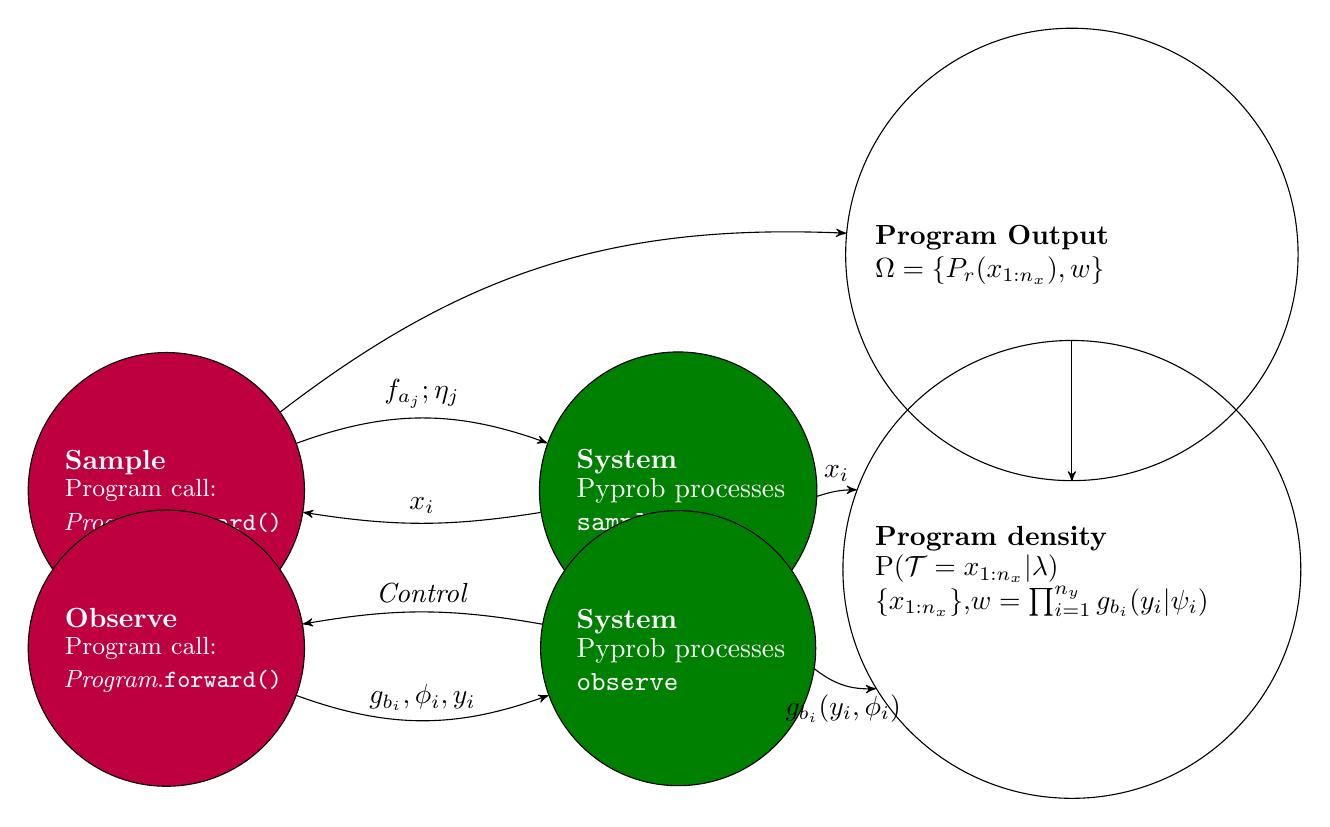
\begin{tikzpicture}[->,>=stealth']

 % Position of Sample 
 % Use previously defined 'state' as layout (see above)
 % use tabular for content to get columns/rows
 % parbox to limit width of the listing
 \node[state,
 text width=3cm, 	% max text width
 yshift=0cm, 		% move 2cm in y
 node distance=0cm, 	% distance to Sample
 anchor=center,
 fill=purple] (Sample) 
{%
\begin{tabular}{l} 	% content
  \textcolor{white}{\textbf{Sample}}\\
  \parbox{4cm}{
  \textcolor{white}{\small{Program call:\\
  \emph{Program}.\texttt{forward()}}}
 }
 \end{tabular}};
  
 \node[state,    	% layout (defined above)
 text width=3cm, 	% max text width
 yshift=-2cm, 		% move 2cm in y
 below of=Sample, 	% Position is to the right of Sample
 node distance=0cm, 	% distance to Sample
 anchor=center,
 fill= purple] (OBSERVE) 	% posistion relative to the center of the 'box'
{%
\begin{tabular}{l} 	% content
  \textcolor{white}{\textbf{Observe}}\\
 \parbox{4cm}{
  \textcolor{white}{\small{Program call:\\
  \emph{Program}.\texttt{forward()}}}
}
\end{tabular}};

 % State: PyProb with different content
 \node[state,    	% layout (defined above)
  text width=3cm, 	% max text width
  yshift=0cm, 		% move 2cm in y
  right of=Sample, 	% Position is to the right of Sample
  node distance=6.5cm, 	% distance to Sample
  anchor=center,
  fill = black!50!green] (PyProb) 	% posistion relative to the center of the 'box'
 {%
 \begin{tabular}{l} 	% content
  \textcolor{white}{\textbf{System}}\\ %system sample
  \parbox{4cm}{\textcolor{white}{Pyprob processes\\ \texttt{sample}}}
 \end{tabular}
 };
 
 % STATE System
 \node[state,
  below of=PyProb,
  yshift=-1cm,
  anchor=center,
  text width=3cm,
  fill = black!50!green] (System) 
 {%
 \begin{tabular}{l}
  \textcolor{white}{\textbf{System}}\\
  \parbox{4cm}{\textcolor{white}{Pyprob processes \\\texttt{observe}}}
 \end{tabular}
 };

 % STATE EPC
 \node[state,
  right of=System,
  yshift = 1cm,
  node distance=5cm,
  anchor=center] (EPC) 
 {%
 \begin{tabular}{l}
  \textbf{Program density}\\
  \parbox{5cm}{P($\mathcal{T}= x_{1:n_x}| \lambda)$\\
  \{$x_{1:n_{x}}\}$,$w= \prod^{n_{y}}_{i=1} g_{b_i}(y_i | \psi_i)$}
 \end{tabular}
 };


  % STATE OUTPUT
  \node[state,
  above of=EPC,
  yshift = -1cm,
  node distance=5cm,
  anchor=center] (OUTPUT) 
 {%
 \begin{tabular}{l}
  \textbf{Program Output}\\
  \parbox{5cm}{$\Omega = \{P_{r}(x_{1:n_{x}}), w\}$}
 \end{tabular}
 };

 % draw the paths and and print some Text below/above the graph
 \path (Sample) 	edge[bend left=20]  node[anchor=south,above]{$f_{a_{j}} ; \eta_{j}$}(PyProb)
 (OBSERVE)     	edge[bend right=20] node[anchor=south,above]{$g_{b_{i}},\phi_i , y_i $} (System)
 (System)       	edge [bend right=20] node[anchor=south,below]{$g_{b_{i}}(y_i, \phi_i)$} (EPC)
 (PyProb)       edge [bend left=9] node[anchor=west, above]{$x_{i}$} (Sample)
 (PyProb)       edge [bend left=9] node[anchor=west, above]{$x_{i}$} (EPC)
%  (System)       	edge [bend left=10]                                          (EPC)
 (EPC)              edge                                                    (OUTPUT)
 (System)  	edge [bend right=10]  node[anchor=north,above]{\emph{Control}} (OBSERVE)
 (Sample)   edge [bend left= 20] (OUTPUT) ;
%  (System)  	edge[loop below]    node[anchor=north,below]{$SC_n\neq 0$} (System)
%  (System)  	edge                node[anchor=left,right]{$SC_n = 0$} (PyProb);

\end{tikzpicture}
\caption{An overview of the hijacking system. $x_i$ represent latent variables. $f_{a_i}$ represent raw sample calls,
$g_{b_j}$ represent conditioning statements. $\mathcal{T}$ corresponds to the program trace. $w$ represents the collective weights. 
$r$ represents run number. $n_x$ represents the number of latent variables and $n_y$ represents the number of
observations, which will always be fixed, but is model dependent. $\lambda$ represents all the other variables generated 
by running the simulator \texttt{.forward()}.
}
\label{fig:systemoverview}
\end{figure}

% In order to correctly characterize this problem we first provide a useful diagram demonstrating 
% the density of the system. 

%  % !TEX root = notes.tex

\tikzset{
    state/.style={
           rectangle,
           rounded corners,
           draw=black, very thick,
           minimum height=2em,
           inner sep=2pt,
           text centered,
           },
}

\begin{figure}
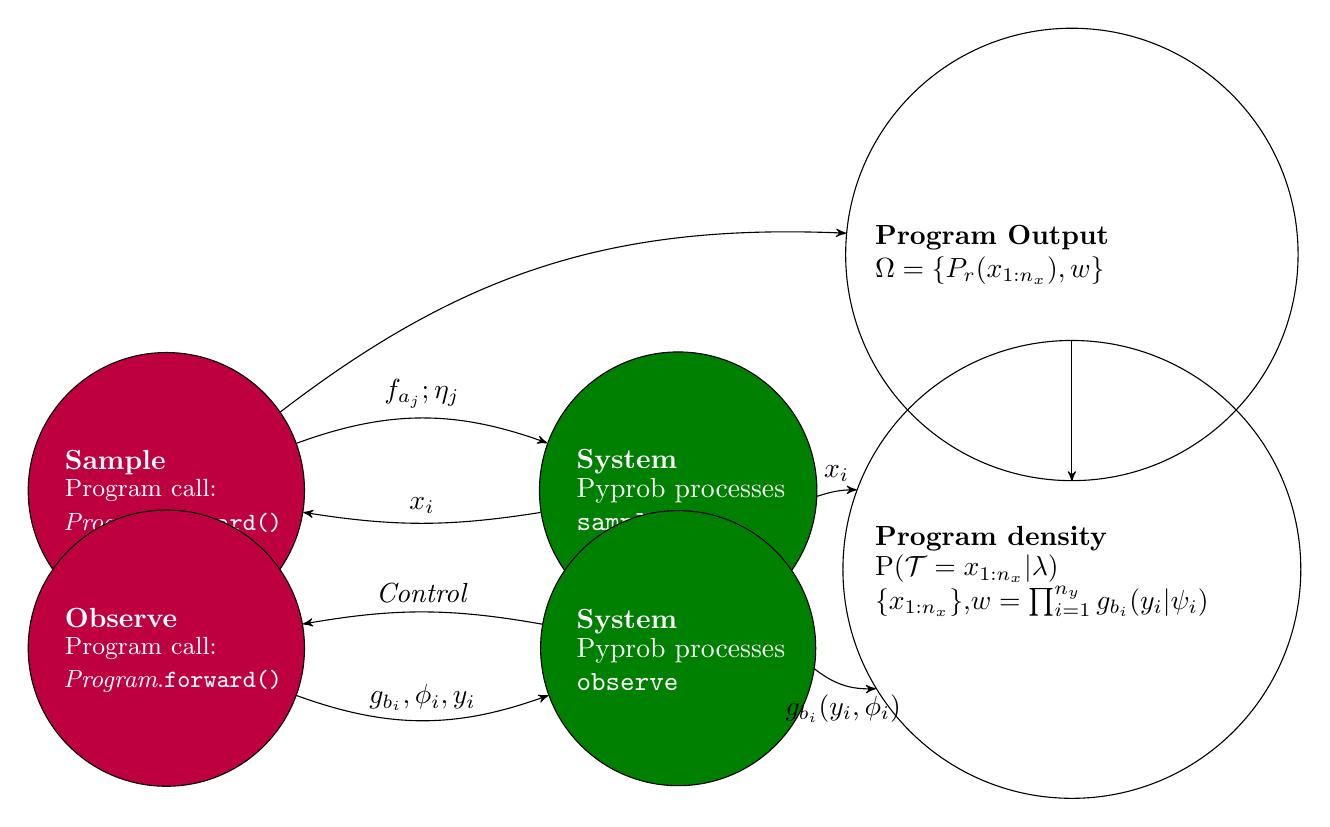
\begin{tikzpicture}[->,>=stealth']

 % Position of Sample 
 % Use previously defined 'state' as layout (see above)
 % use tabular for content to get columns/rows
 % parbox to limit width of the listing
 \node[state,
 text width=3cm, 	% max text width
 yshift=0cm, 		% move 2cm in y
 node distance=0cm, 	% distance to Sample
 anchor=center,
 fill=purple] (Sample) 
{%
\begin{tabular}{l} 	% content
  \textcolor{white}{\textbf{Sample}}\\
  \parbox{4cm}{
  \textcolor{white}{\small{Program call:\\
  \emph{Program}.\texttt{forward()}}}
 }
 \end{tabular}};
  
 \node[state,    	% layout (defined above)
 text width=3cm, 	% max text width
 yshift=-2cm, 		% move 2cm in y
 below of=Sample, 	% Position is to the right of Sample
 node distance=0cm, 	% distance to Sample
 anchor=center,
 fill= purple] (OBSERVE) 	% posistion relative to the center of the 'box'
{%
\begin{tabular}{l} 	% content
  \textcolor{white}{\textbf{Observe}}\\
 \parbox{4cm}{
  \textcolor{white}{\small{Program call:\\
  \emph{Program}.\texttt{forward()}}}
}
\end{tabular}};

 % State: PyProb with different content
 \node[state,    	% layout (defined above)
  text width=3cm, 	% max text width
  yshift=0cm, 		% move 2cm in y
  right of=Sample, 	% Position is to the right of Sample
  node distance=6.5cm, 	% distance to Sample
  anchor=center,
  fill = black!50!green] (PyProb) 	% posistion relative to the center of the 'box'
 {%
 \begin{tabular}{l} 	% content
  \textcolor{white}{\textbf{System}}\\ %system sample
  \parbox{4cm}{\textcolor{white}{Pyprob processes\\ \texttt{sample}}}
 \end{tabular}
 };
 
 % STATE System
 \node[state,
  below of=PyProb,
  yshift=-1cm,
  anchor=center,
  text width=3cm,
  fill = black!50!green] (System) 
 {%
 \begin{tabular}{l}
  \textcolor{white}{\textbf{System}}\\
  \parbox{4cm}{\textcolor{white}{Pyprob processes \\\texttt{observe}}}
 \end{tabular}
 };

 % STATE EPC
 \node[state,
  right of=System,
  yshift = 1cm,
  node distance=5cm,
  anchor=center] (EPC) 
 {%
 \begin{tabular}{l}
  \textbf{Program density}\\
  \parbox{5cm}{P($\mathcal{T}= x_{1:n_x}| \lambda)$\\
  \{$x_{1:n_{x}}\}$,$w= \prod^{n_{y}}_{i=1} g_{b_i}(y_i | \psi_i)$}
 \end{tabular}
 };


  % STATE OUTPUT
  \node[state,
  above of=EPC,
  yshift = -1cm,
  node distance=5cm,
  anchor=center] (OUTPUT) 
 {%
 \begin{tabular}{l}
  \textbf{Program Output}\\
  \parbox{5cm}{$\Omega = \{P_{r}(x_{1:n_{x}}), w\}$}
 \end{tabular}
 };

 % draw the paths and and print some Text below/above the graph
 \path (Sample) 	edge[bend left=20]  node[anchor=south,above]{$f_{a_{j}} ; \eta_{j}$}(PyProb)
 (OBSERVE)     	edge[bend right=20] node[anchor=south,above]{$g_{b_{i}},\phi_i , y_i $} (System)
 (System)       	edge [bend right=20] node[anchor=south,below]{$g_{b_{i}}(y_i, \phi_i)$} (EPC)
 (PyProb)       edge [bend left=9] node[anchor=west, above]{$x_{i}$} (Sample)
 (PyProb)       edge [bend left=9] node[anchor=west, above]{$x_{i}$} (EPC)
%  (System)       	edge [bend left=10]                                          (EPC)
 (EPC)              edge                                                    (OUTPUT)
 (System)  	edge [bend right=10]  node[anchor=north,above]{\emph{Control}} (OBSERVE)
 (Sample)   edge [bend left= 20] (OUTPUT) ;
%  (System)  	edge[loop below]    node[anchor=north,below]{$SC_n\neq 0$} (System)
%  (System)  	edge                node[anchor=left,right]{$SC_n = 0$} (PyProb);

\end{tikzpicture}
\caption{An overview of the hijacking system. $x_i$ represent latent variables. $f_{a_i}$ represent raw sample calls,
$g_{b_j}$ represent conditioning statements. $\mathcal{T}$ corresponds to the program trace. $w$ represents the collective weights. 
$r$ represents run number. $n_x$ represents the number of latent variables and $n_y$ represents the number of
observations, which will always be fixed, but is model dependent. $\lambda$ represents all the other variables generated 
by running the simulator \texttt{.forward()}.
}
\label{fig:systemoverview}
\end{figure}


\section{Amortized Rejection Sampling}

One common problem in traditional simulators, \emph{programs}, outside of the standard probabilistic
programming framework is that they rely heavily on rejection sampling 
to generate samples from the target density. Not only is rejection sampling 
computational inefficient, [especially if criteria in which samples are generated
has been poorly calibrated] (may leave out this statement as it may make a reviewer
question why would amortization work any better.), but it creates complications for inference.
As the rejection sampling loops provide no explicit form of the target density,
we can not simply evaluate the density and leverage statistically and computationally
efficient algorithms such as MCMC sampling. This inhibits our ability to transform an arbitrary
stochastic simulator into a probabilistic programming framework~\cite{baydin2018efficient}. 
To this end, we derive both a mathematical and engineering based framework to facilitate 
the amortization of rejection sampling loops in arbitrary simulators, which provides a path
way to both leverage a larger, more efficient class of inference methods and convert arbitrary
stochastic simulators into probabilistic programs systems.

\subsection{Rejection Sampling}

Rejection samplers are heavily used when designing simulators [ add SHERPA etc], due to their ease of use and ability to model 
any arbitrary distribution on $\mathbb{R}^{D}$, with a sufficiently well designed rejection sampling scheme~\cite{MEYER20083408,martino2012improved,casella} 

In the standard setting we let $X$ be a random variable whose density is $f(x)$ that we cannot easily 
sample from, but can evaluate. Using a random variable $Z$, whose density is $g(z)$  that we can efficiently
sample from, then we can generate a sample $X$ by sampling $Z$ and accept $Z$ with probability
$p_{accept} = \frac{f(x)}{Mg(x)}$, which we can do until acceptance. 
M is constant that has a finite bound, $M \in (1, \infty)$, on the likelihood ratio $\frac{f(x)}{g(x)}$ over the 
support of $X$. $M$ must also satify the following inequality $f(x) \leq M g(x)  \forall x$. 
This implies that the support of $Z$ must also contained the support of $X$, that is
$g(x) > 0$ whenever $f(x)>0$. 
The standard algorithm is defined as follows:
\begin{algorithm}
  \small
   \caption{Rejection Sampling}
    \begin{algorithmic}\small
       \State {At iteration $i$ s.t $i \geq 1$}
       \State $X_{i} \sim g(X_{i})$ 
       \State $U_{i} \sim \mathcal{U}(0,1)$
       \If{$U_{i} \leq M \frac{f(X_i)}{g(X_{i})}$}
       \State{ accept $X_i \sim f$}
       \Else
       \State{$i \gets i + 1$, repeat}
       \EndIf
\end{algorithmic}
\end{algorithm}

As useful rejection sampling is, it has many short comings. 
In particular, to simulate proposals for certain distributions,
such as truncated normal distributions, regardless of the easy to sample from proposal
chosen the computational running time of such rejection statements can be shown to have an
expectation equal to infinity. Thus, the ability to learn and replace such rejection
sampling blocks with learnt surrogate functions, that are expressive enough to 
reciprocate the behavior of the rejection sampling block buys the user two things. 
A) It reduces the computational complexity of the simulator. 
B) As we now have a direct functional form of the density, we can correctly leverage
more computationally and sample efficient inference schemes. 

\begin{figure}
  % \begin{minipage}[c]{0.67\textwidth}
  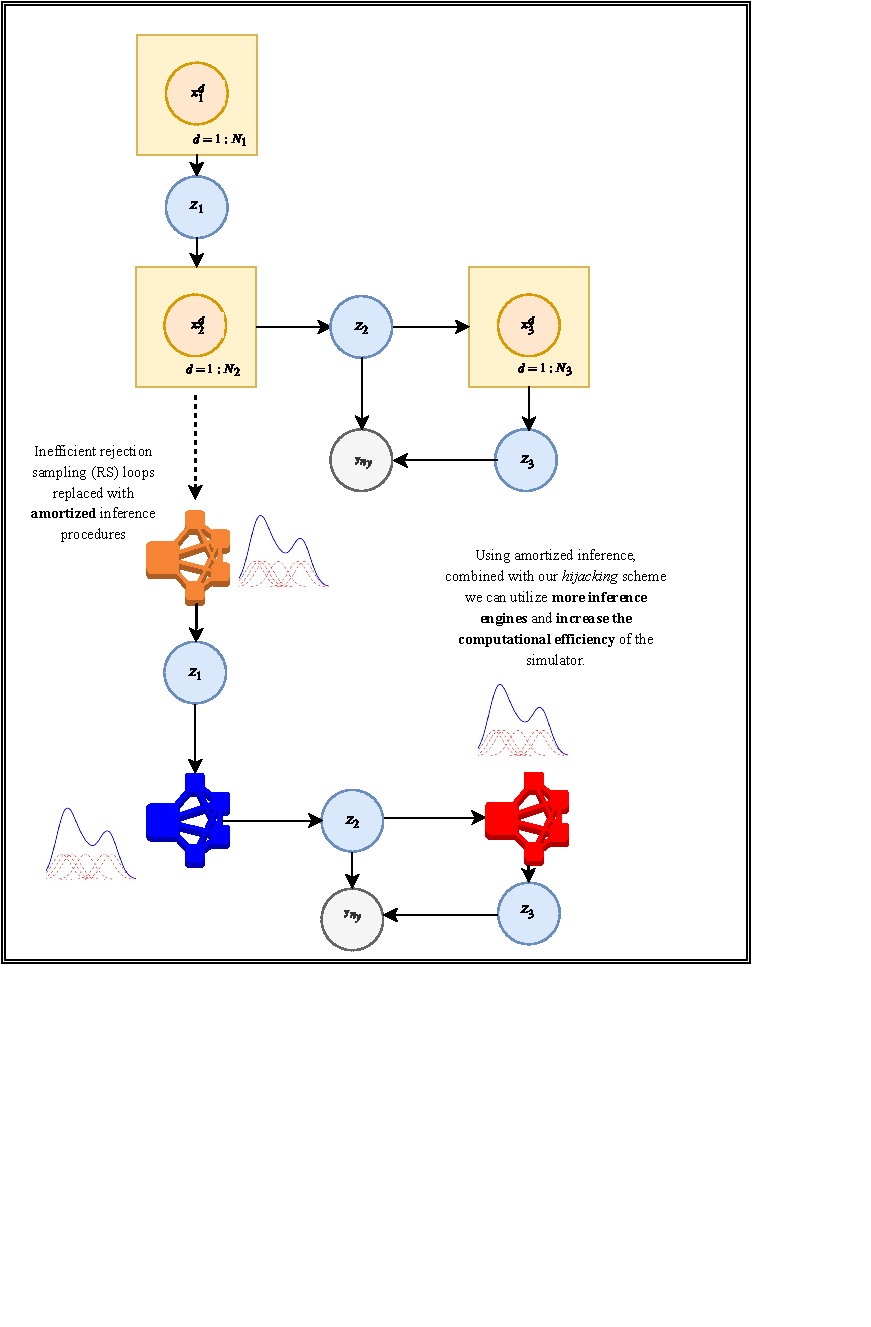
\includegraphics[width=0.6\textwidth, height=0.6\textheight,keepaspectratio]{amoritized_rejection.pdf}
  % \end{minipage}\hfill
  % \begin{minipage}[c]{0.3\textwidth}
    \caption{Using PyProb we can locate all regions of inefficient sampling 
    and replace those points in the code with learnt functions that represent
    the distributions of the rejection sampling statements. $Z_{i}$ represents the marginal and 
    by learning surrogate functions for each of the rejection sampling loops.
    In doing so we can learn approximate raw sample distributions $f(x_{i} | \eta)$ for each
    rejection sampling loop. This means that we can evaluate the function at each part in the simulator, enabling
    us to construct a target density that can be evaluated when using MCMC inference schemes such as RMH.}
    \label{fig:amortized_sampling}
  % \end{minipage}
\end{figure}


We do this by replacing the rejection sampling blocks with 
learnt functions from an amortized inference procedure Figure~\ref{fig:amortized_sampling}.
This then enables us to replace rejection sampling loops with amortized functions that 
are quick to evaluate, provide a functional form to the density and significantly reduce 
memory over-heads, as compared to~\cite{baydin2018efficient}, due to not having to track the 
thousands of raw sample calls $f_{a_i}$ generated in standard simulators. 

Consider the following program, that is representative of a simple stochastic simulator
and two types of rejection sampler:


\noindent
\begin{tabular}{|p{3.6cm}|p{3.6cm}|p{3.6cm}|}
\hline
Stochastic Simulator  & Rejection Sampler 1 & Rejection Sampler 2 \\
\hline
\begin{lstlisting}[mathescape=true]
    def f():
      $z_{1} \sim \mathcal{N}(0,1)$
      $z_{2} \gets R_{1}(z_1, 1)$
      $z_{3} \sim \mathcal{U}(0,2)$
      $z_{4} \gets R_{2}(z_2,z_3, 1)$
    return $g(z_{1:4})$
\end{lstlisting}&
\begin{lstlisting}[mathescape=true]
def $R_1(z_1)$:
  $x \sim \mathcal{N}(z_1,1)$
  if $x > 0$:
    return $x$
  else:
    return $R_{1}(z_1)$
\end{lstlisting}&
\begin{lstlisting}[mathescape=true]
def $R_2(z_2, z_3)$:
  $y \gets 0$
  while $y < z_2$:
    $y \sim \mathcal{N}(z_3,1)$
  end
  return $y$
\end{lstlisting}\\
\hline
$P(\mathcal{T}= x_{1:n_x} | \lambda)$ & $q_{1}(z_{2} | z_{1})$ & $q_{2}(z_{4} |z_{2},z_{3})$ \\
\hline
\end{tabular} 

Here the rejection sampling functions take an additional argument $1$, or $0$,
to specify whether or not we want to collect samples to train, $1$, else replace with 
the learnt function, $0$. $P$ represents the program density and $q_{1}$ and $q_{2}$ represents 
the unknown densities that we wish to learn through an amortized approach.
It is important to note that the expected running time of the rejection sampler is expected to geometric mean, we can show this as follows:
\textbf{Bradley:  You only arrive at this, if the density is uniform}
\begin{align*}
P( X= x) = \sum^{\infty}_{n=1} P(\text{reject $n-1$ times}, \text{draw} Y = x) \\
\text{todo} 
\end{align*}

In addition to this, if we have direct access to a rejection sampling loop then it is indeed 
possible to construct the density, up to a constant of proportionality. 
That is:
\begin{align*}
y \sim q(\theta) \\
do something \\
\alpha = p_{accept}(y,\theta) \\
\mathtt{if} Bern(\alpha) = 1: \\
return y
\end{align*}
thus the density of $y,\theta \propto q(\theta) \alpha$.
However, in order to do construct this we need the input $\theta$, $y$, $\alpha$ and the distributions utilised for the rejection sampling loop. 
For any arbitrary simulator, written in a generic code base, this is an incredibly hard 
task to do, because rejection sampling blocks within simulators are not necessarily written in a standard template
\textbf{Add examples in a supplement.  Need to demonstrate to YW that this is challenging to do, even if you know where 
the rejection sampling loops are. Hypothesis, RS loops are not written in a templated form}. With the PPX protocols previously developed in \cite{baydin2018efficient,gram2019hijacking} we can however, 
extract all variables, other than $\alpha$ in an automated way.
However, without being able to easily extract $\alpha$ this means that we are unable to 
correctly build the form of the density and thus we limited in our ability to leverage 
powerful inference methods such as MCMC and Variational inference.
Thus, we propose another approach, automating the amortization of rejection sampling loops. 
To learn functions that we can easily sample from and use to construct the density of the entire
simulator. 


The simulated densities for both each rejection sampling block can be seen in Figure~\ref{fig:rs_simulated}.
\begin{figure}
  \centering
  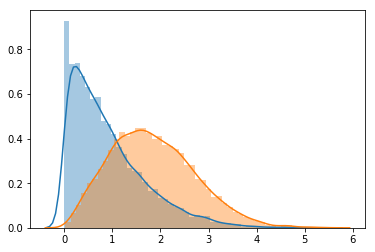
\includegraphics[width=0.2\textwidth, height=0.2\textheight, keepaspectratio]{rs_plots.png}
  \caption{ Simulated densities for rejection sampling block 1, \emph{blue} and rejection
  sampling block 2, \emph{orange}.}
  \label{fig:rs_simulated}
\end{figure}

In order to replace such rejection sampling blocks with learnt functions that we 
can efficiently sample from, we must correctly specify our variational objective.

\subsection{Constructing the Objective}

The framework we present in this section is generally applicable to stochastic simulator 
environment, where there exists rejection sampling loops. 

We start by noting that the prior, defined in the context of the outer samples is 
defined as: 
\begin{equation}
  p(x) = 
  \begin{cases}
    \prod^{n_{x}}_{j=1} f_{a_j}(x_j ; \psi_j) if \mathcal{B}(x) = 1 \\
    0
  \end{cases}
\end{equation}
We start with the information projection we construct the variational objective as follows:
\begin{align*}
  J(\eta) = KL(p(x) || q(x; \eta)) \\
   = \int p(x)\ln\left(\frac{p(x)}{q(x;\eta)}\right) dx \\
  %  \int p(x')dx' \gets 1 \\
  %  &= \mathbb{E}_{p(x)}[\ln(p(x))]  - \mathbb{E}_{p(x)}[\ln(q(x;\eta))]\\
  %  &= \ln(1) -  \mathbb{E}_{p(x)}[\ln(q(x;\eta))]\\ % I do not agree with this line
  %  &= -\mathbb{E}_{p(x)}[\ln(q(x;\eta))] \\
  %  &= -\mathbb{E}_{p(x)}[\sum^{n_x}_{j=1}\ln(q_{a_j}(x_j;\eta))] \\
   \text{Let } a_{j} \in \{1, \ldots, L\} , S_{R} \subset \{1, \ldots, L\} \\
   = \cancelto{\text{no dependence on } \eta}{\mathbb{E}_{p(x)}[\sum^{n_x}_{j=1,a_j \notin S_{R}}\ln(p(x))]}-\mathbb{E}_{p(x)}[\sum^{n_x}_{j=1,a_j \in S_{R}}\ln(q_{a_j}(x_j;\eta))]\\
\end{align*}

Thus, to define the objective for each subproblem $r  \in S_{R}$ as:
\begin{equation}
  \label{eq:objective}
  J_{r}(\eta_r) = -\mathbb{E}_{p(x)}[\sum^{n_x}_{j=1}\mathbb{I}(a_j = r)\ln(q_r(x_j;\eta_r, \phi_j))]
\end{equation}

where during training we extract samples from each forward run and train each rejection sampler
separately. 


\section{Experiments: Amortizing Stochastic Processes}

\paragraph{TODO list}
\begin{itemize}
  \item Implement baselines
  \item Implement plotting scripts and evaluation scripts
  \item testing code and infrastructure
  \item litrature review on any methods to learn rejection sampling methods, 
  and conditional density estimation. See this paper for kernel approximation 
  methods~\cite{erraqabi2016pliable}. In addition to the methods listed in the 
  rejection sampling subsection. 
\end{itemize}

\paragraph{Tom Questions}

\begin{itemize}
  \item I don't understand how the objective function is comparing the generated samples from the density 
  estimator to the ground truth, at least in the way it is currently defined? 
  \item All RS references I look at state that we must sample from a uniform distribution and
  then check if our proposed value is less than that uniformly sampled point, yet our RS do not have this,
  nor what is the acceptance probability within our rejection sampling statements? The proof for rejection sampling seems to rely on the fact that you are drawing from a uniform distribution.  

  \end{itemize}
\subsection{Ground truth}

Because in this simple case we have direct access to $\alpha$, the rejection sampler acceptance probability,
we can calculate the true density up to a constant of proportionality. 
\textbf{I will add this tomorrow}. I had no idea about this, until my meeting with 
YW today. 

\subsection{Baseline}
As a first approach, we train a regressor to learn a function to map
between the input / output pairs that are outputted from the rejection
sampling blocks with in the simulator. 

For $R1$ we have one input $z^{r1} \in \mathbb{R}^{1 \times 1}$ and one output $y^{r1} \in \mathbb{R}^{1 \times 1}$.
For $R2$ we have two inputs $z^{r2} \in \mathbb{R}^{2 \times 1}$ and one output $y^{r2} \in \mathbb{R}^{1 \times 1}$.
For training purposes we generate $n_{b}$ batches of $n_{t}$ samples for training. 
This means that $z^{r1}_{batch}\mathbb{R}^{n_{b} \times 1}$. 
For the loss function we use a simple mean squared error loss \textbf{We can try different loss 
functions and optimizers} and use the
neural network, $\Gamma(z, y)$, to learn a $\hat{\mu}$ and $\hat{\sigma}^{2}$ to parametize 
a normal proposal. For $R1$, this means $\Gamma_{r1}(z,y) \rightarrow \hat{\mu_{r1}},  \hat{\sigma_{r1}}^{2}$  
and so the proposal $q(z_{1} | z_{2}) = \mathcal{N}(\hat{\mu_{r1}},  \hat{\sigma_{r1}}^{2})$. 
Once learned we can then efficiently sample from the parameterized normal distribution, which
represents the density of the sub-program represented by $R1$. 
This is then replaced in the simulator, during inference time. 

\paragraph{observations} As the functions are relatively simple the loss functions it gets t
to a loss of around 0.6 and stops decreasing. Although, this seems low, I don't think that it is
actually good, because that would mean on average, for each data point there is a loss of $\pm$ 0.6
which per data point is quite bad. That may be for a number of reasons, using MSE loss, using a simple
model architecture. It really struggles to model the tails. It may require a much larger batch input size. 
. Increasing the batch size helped to correct for the peaked density, however the behavior is still odd.
The peaked behaviour still does not disappear, this, I believe is due to the loss function averaging 
over all points.



 \textbf{Add results from current experiments}


\subsection{2nd Baseline}
Instead of using a single Gaussian, use a proposal that is a mixture of Gaussians. 
That is, for $R1$,   $q(z_{1} | z_{2}) = \sum^{N}_{i=1}K_{i}\mathcal{N}(\hat{\mu^{i}_{r1}},  \hat{\sigma^{i}_{r1}}^{2})$
under the constraint that $\sum^{N}_{i=1}K_{i} = 1$. Maybe $N$ can be treated as a hyper-parameter. 
Or choose particular values.
\subsection{More complicated: Conditional Density estimation}

\subsection{3rd Baseline}
 
Use the variational objective constructed above. 

\paragraph{Normalizing flows} One recent technique for density estimation, in the amortized inference setting,
is normalising flows combined with variation inference~\cite{rezende2015variational}.
Flow-based methods work by leveraging a simple property of differential geometry applied 
to random variables. 
That being the change of variables. 
Using flow based methods we can construct our rejection sampling block density, by learning a flow to map from
a simpler distribution to more complicated one.
Let $z \sim r(z)$ where $r(z)$ represents the posterior defined by the rejection
sampling loop, and define $\pi$ to be a smooth and invertible function.
When $\pi$ acts $z$ we transform the random variable from one domain, to another. 
Thus, if $z\prime = \pi(z)$ then we can construct the density of  
the probability density of the new random variable $z\prime$ under the flow initiated by $\pi$: 
\begin{equation}
r(z\prime) = r(\pi^{-1}(z\prime)) \left|\det \frac{\partial \pi^{-1}}{\partial z'}\right| = r(\pi^{-1}(z\prime)) \left|\det \frac{\partial \pi}{\partial z\prime}\right|^{-1} 
\end{equation}

Flows available are Real-NVP~\cite{dinh2016density} and Neural Spline flows~\cite{durkan2019neural}.
There are several others, for other techniques ask Gunes. 

\begin{itemize}
  \item Do we need to know the base distribution that the RS block is sampling from? i.e there maybe be multiple $r(z)$ in each 
  RS block. 
  \item Is it right to say here that $z\prime$ is the output of the RS block, we do not know $\pi$ here, or is $r(z)$ the raw sample $f_{a_i}$ and $\pi$ the distribution specified by the rejection sampling loop? 
  \item We need to learn $\pi(.)$
\end{itemize}
\subsection{Using variants of VAEs}

Notes from models that define an explicit,  
tractable density are highly effective, 
because they permit the use of an optimization algorithm directly on the log-likelihood of the training data.
However,  the  family  of  models  that provide  a  tractable  density  is  limited,
with  different  families  having  different disadvantage.
The rejection sampling loops, if proposed correctly, provide a way of generating 
samples from some density, but do not provide a way of constructing the target density (\textbf{Bradley: Ask Tom, is this true?}). 
Within event and population-based simulators, the rejection sampling loops have been designed with care,
to ensure that they are representative to the events that they are simulating. So we can, with confidence,
assume that they are representative of some density. 
However, to utilise powerful inference engines, we must be able to construct the 
full density of the program. 




\section{ Questions for Tom}

\textbf{New questions to ask Tom}

\begin{itemize}
  \item How is Equation~\ref{eq:}
  \item Isn't what we are doing just conditional density estimation? It seems
  like there is a lot of prior work here. I.e see this paper here for a good overview ~\cite{greenberg2019automatic}
  \item It does seem like this field has a large extensive past, but we still have a small niche.
\end{itemize}

\textbf{Old questions for Tom}
\begin{itemize}
  \item Whilst the variational posterior we choose as our proposal has a functional form  
  and can be sampled, the functional form of the rejection sampling loops is not explicitly known,
  which leads to problems when calculating the $KL$-divergence - reparametrize a with a function from a family of easy to sample distribution. 
  \item There are two approaches that we can take to calculating some divergence metric. 
  \item 1) Using something like a non-parametric divergence estimator that makes use of Renyi and $L_{2}$ divergences (see \cite{basseville2013divergence} for details) - No point, more difficult to implement
  \item 2) Use some form of kernel density to estimation to approximate the functional form of the rejection sampling 
  block, which can be used in place. From which we learn a variational approximation characterized by a trained network that we can sample from quickly. 
  \item An issue with approach 2) is that if I can approximate the density in functional form aren't there more efficient methods that we can use? - There are other methods out there and it would maybe make sense to compare some of those methods. However, it may still be difficult to sample. 
  \item Or, if assuming that the rejection sampling block can be arbitrary dimension, are we first learning a flow to represent that density and then learn a variational approximation of something that we can easily sample from. 
  \item But, this is very much the idea behind normalising flows, take a simple distribution that you can sample and then map it to the ``complicated'' density - Question not well defined. 
  \item Stein Variational inference may be quite nice to use here~\cite{feng2017learning}, but it does make explicit assumptions in requiring the densities to be differentiable. - Yes this metod is good, but only works in the continuous domain. 
  \item  For an overview of all variational methods, including the use of different divergence metrics see here ~\cite{8588399} - Answered - Quite finickity to set up. 
\end{itemize}

\section{Additional TODOs}


\begin{itemize}
\item Before implementing such tools into the simulator, spend time looking for simpler stochastic simulators 
that can be hijacked but have target densities that can be constructed analytically. 
\item If we are not utilizing the additional information stored in the trace, which is only used during the inference compilation
training procedure, then we do not need it all, as for importance sampling we only require the weights after each \texttt{forward()}
update. 
\item If we cannot find any pre-existing simulators that are amenable to this approach then, we need to create our own, with
a rejection sampling loop, that can be exploited by the new machinery. This would enable us to debug, provide a simple example 
for the paper and understand the feasibility of the entire approach. 
\end{itemize}

\bibliography{refs}
\bibliographystyle{plain}
\appendix

\section{The unconditional acceptance probability}

Given a collection of i.i.d random variables $\{X_{i}\}_{i = 1:n}$ with 
cumulative density function (CDF) $F_{X}$. Then by the Glivenko-Cantelli theorem~\cite{tucker1959generalization} 
we can define the empirical distribution function for $x \in \mathbb{R}$ as:
\begin{equation}
  F_{n}(x) = \frac{1}{n}\sum^{n}_{i=1} \mathbb{I}_{[X_{i}, \infty)}(x)
\end{equation}
And for any fixed $x \in \mathbb{R}$, the Strong law of large numbers ensures that 
$F_{n}(x) \rightarrow F_{X}(x)$ as $n \rightarrow \infty$ as 
\begin{equation}
\mathbb{E}[\mathbb{I}_{[X_{i},\infty)}(x)] = 
 P[\mathbb{I}_{X_{i},\infty)}(x) = 1] = P[X_{i}\leq x] = F_(X)(x)
\end{equation}
where $\mathbb{I}_{A}(x)$  is the indicator function for a set $A$. 

\begin{align}
  \text{Prob}(U \leq \frac{p_{X}(z)}{Mg_{Z}(z)} = \mathbb{E}_()
\end{align}
\section{Law of total expectations}

If $X$ is a random variable whose expected value is $\mathbb{E}[X]$ and $Z$ is a random variable on the same probability space
then: \begin{equation}
  \label{eq:lawoftotalexp}
  \mathbb{E}[X] = \mathbb{E}_{p(z)}[\mathbb{E}_{p(x|z)}[X | Z]]
\end{equation}
That is, the expected value of $X$ given $Z$ is the same as the expectation of $X$.

\section{Limitations with different inference engines}  


\subsection{Prior based sampling}
In prior based sampling we take our existing program and look directly at the product of all the raw sample calls, denoted $f_{a_i}(x_i | \eta)$ and 
construct a proposal that is is dependent on those. In this sampling scheme our proposal is defined as:
\begin{equation}
  q(x_{1:n_{x}}) = 
  \begin{cases}
    \prod_{i=1}^{n_x} f_{a_i}(x_i | \eta) \hspace{0.1cm} \texttt{if} \hspace{0.1cm} \mathcal{B}(x_{1:n_{x}})=1 \\
    0
  \end{cases}
\end{equation}
where $\mathcal{B}(\cdot)$ is satisfied by the simulator and $f_{a_i}(\cdot)$ represents a
raw random sample, $\eta$ is a subset of the variables in-scope at the point of sampling
and $n_{x}$ is the number of latent variables.
 This is true in all inference engines used in this hijacking framework.
However, this makes use of no conditioning and is not sufficient for performing inference in
complex, population-based simulations.

\subsection{Non-prior Based Sampling}
In non-prior based sampling we utilise conditioning too, which enables 
us to explore spaces more efficiently. 
In the current hijacking set-up, we
can only do conditioning at the end of each \texttt{forward()} run of the simulator. 
This does inhibit certain inference engines and makes aspects of performing inference 
within this setting more complicated. 
Nonetheless, there are several inference schemes 
that we can exploit and utilise. 
We shall now give an Introduction to each of these schemes. 


\subsection{Importance Sampling}
In the generalised probabilistic programming setting an importance sampling scheme over the 
program raw samples and observations can be defined as follows:
\begin{equation}
  \label{eq:posterior}
  p(\mathcal{T}=x_{1:n_x}| \lambda)=
  \begin{cases}
  \prod_{i=1}^{n_x} f_{a_i}(x_i | \eta) \prod_{j=1}^{n_y} g_{b_j}(y_j | \phi) \hspace{0.1cm} \texttt{if} \mathcal{B}(x_{1:n_x}) = 1\\
  0
  \end{cases}
\end{equation}

where the observe statements are defined by $g_{b_j}(.)$, $\phi$ plays the same role as 
$\eta$ and $n_y$ represents the number of observations.
The expectation over the whole program can be defined as: 
\begin{equation}
\mathbb{E}_{p(\Omega | \lambda)}[h(\Omega)] = \mathbb{E}_{p(x_{1:n_x} | \lambda)}[h(P_r(x_{1:n_x}))]
\end{equation}
\textbf{Note: It is a little weird how we define this, as the the program output $\Omega$ should
also include the product of the weights}

where $r$ represents a run of the program, $P_{r}(\cdot)$ is the entirety of the program output,
$h(\cdot)$ is just a deterministic function. 

As the importance sampler updates the weights according to the following formula:
\begin{equation}
  w(x_{1:n_x}) = \prod^{n_x}_{i=1}\frac{f_{a_i}(x_i | \eta_i)}{q_i(x_i |f_{a_i}, \eta_i)} \prod^{n_y}_{j=1} g_{b_j}(y_j | \phi_j)
\end{equation}

When the number of observations is fixed, the combined weight is equal to $w(x_{1:n_x}) = \prod^{n_y}_{j=1} w_j $. 
To generate the weight up to each observe we can define $K(j)$ to be a function that returns the least $i$ before hitting an observe $j$.
This enables us to write the $j$-th weight as follows:
\begin{equation}
  w_j(x1:K(j)) = g_{b_j}(y_j | \psi_j) \prod^{K(j)}_{K(j-1)+1} v_i
\end{equation}
where we define $v_j = \frac{f_{a_j}(x_j | \eta_j)}{q_j(x_j |f_{a_j}, \eta_j)}$

Taking these definitions we can construct a target density over the 
latents that is proportional to the products of \texttt{sample} and \texttt{observe}
statements \textbf{Note: Add update posterior here}.
Thus, given the proposal $q(x_{1:K(t)})$ we define the importance weight as:
\begin{multline}
  w(x_{1:t}) = \prod^{t}_{j=1} w_j (x_{1:K(j)}) = \\
   \frac{p_t(x_{1:K(t)})}{q(x_{1:K(t)})} =
 \begin{cases}
  \prod^{t}_{j=1}g_{b_j}(y_j | w_i)\prod^K(j)_{K(j-1)+1} v_i \hspace{0.1cm} \texttt{if} \hspace{0.1cm} B_t(x_1:K(t))=1 \\
  0
 \end{cases}
\end{multline}

One problem with importance sampling is in its ability to scale and condition upon multiple observations. |
Choosing a \emph{good} prior remains challenging. 

\subsection{Sequential Monte Carlo}
Given multiple observations, we can ake the inference more computationally efficient 
by employing sequential monte carlo (SMC), although as we can only condition at the end 
of one full run of the simulation, computational speed increases are minimal.
SMC allows for conditioning on multiple observations, but the number of observations must
be fixed. \textbf{Note: If we could condition on observations within the simulator, we 
could get dramatic speed increases over standard importance sampling.We can actually do this 
in pyprob, but it requires knowing where to condition. That can be quite challenging 
for arbitrary code. }


\begin{algorithm}
    \caption{SMC for Population Based Simulators - well any general program - not new}
    \label{alg:euclid}
    \begin{algorithmic}[1] % The number tells where the line numbering should start
        \Procedure{SMC}{$T,M$,\textbf{x}, \textbf{w},\textbf{v}, \textbf{g}}
          \For{$t = 1:T$}
            \For{$m = 1:M$}
              \State $w^{m} = 1  $
              \For{$k = K(t-1)+1:K(t)$}
                \State $x^m_k \sim q_k(x^m_k | f_{a^{m}_{k}},\eta^{m}_{j})$
                \State $w^m_t \gets w^t_m v_j^m(x_k^m)$
                \EndFor
            \EndFor
          \State $w^m_t \gets w^m_t g_{b_{t}^m}(y_t^m | \psi^m_t)$
          \State $\{x^{1:m}_{1:t}\}$ $\gets$ \texttt{resample}( $\{x^{1:m}_{1:t}\}$,  $\{w^{1:m}_{1:t}\}$ )
        \EndFor
        \EndProcedure
    \end{algorithmic}
\end{algorithm}

To implement SMC in the current set-up we round require a forking method and the 

\subsection{Random-walk Metropolis Hastings}

Due to the current set-up performing Random-walk Metropolis Hastings (RMH) is not feasible 
as the rejection sampling blocks within the simulator mean that we cannot correctly perform RMH
as we do not have a functional form for all parts of the simulator to construct a target density
that we can evaluate. \textbf{Note:
Ask tom what:  one can sometimes achieve improvements by instead using the type of the distribution object 
associated with $x_m$ (what does this first part mean?) 
 to automatically construct a valid random walk proposal that allows for improved
 hill climbing behavior on the individual updates. }. 

\textbf{TODO: Add some of the plots generated from this model and an accompanying analysis to them.}
 

\section{An Example: Modelling Parasite Densities in Simulation}
% \begin{wrapfigure}{r}{0.4\textwidth}
  \begin{figure}[h!]
    \centering
    \label{fig:parasite}
    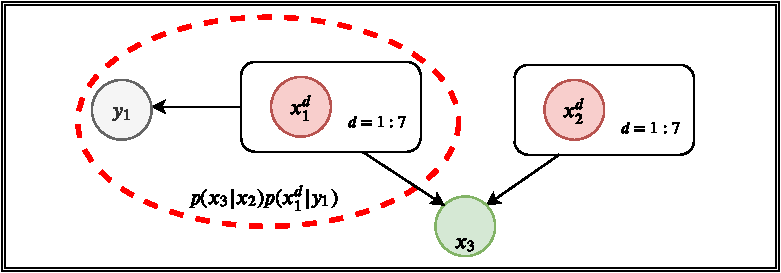
\includegraphics[width=0.4\textwidth]{parasite_model.pdf}
    \caption{The DAG of the Parasite model.}
  % \end{wrapfigure}
  \end{figure}
The parasite model by Smith el al.~\cite{smith2006relationship} is a simple stochastic 
model for determining the number of infections within a given population demographic.
The models hypothesized in ~\cite{smith2006relationship} were found, 
after extensive testing and development, to not characterise well the number 
of infections among different demographics, especially those under 15 years old. 
By using probabilistic programming we can immediately understand 
the expressiveness of the proposed model and can exact important insights for 
extending the proposed models, which increases ones ability to develop 
improved models to estimate parasite densities, given 
our observations of the seasonal entomological inoculation rate (EIR).
In addition to this we can greatly reduce the computational costs, whilst
improving model comprehension and expressivity.  


\paragraph{Common features of the models}
The models used are all discrete time micro-simulations of malaria in humans, 
based on the published model used in[1], which we refer to as the base model.
The model for infection of the vector as a function of parasite densities[2] 
(and hence for the effect of vaccination on onward transmission), the case-management model[3], 
the model of vaccination by pre-erythrocytic vaccines[4], the models for clinical outcomes and mortality[5,6], 
and the basic design of the scenarios used for predicting impacts[3,7] all correspond to the previous descriptions,
 which are accompanied by detailed rationales for the formulations used.  

For all models, the number of infections  introduced in individual $i$ in five-day time step $t$, is distributed as:
\begin{equation}
  h(i,t) \sim \textit{Pos}(\lambda(i,t))
\end{equation}
where the expected number $\lambda(i,t) = S(i,t)E_a(i,t)$ and $S(i,t)$ is the suseptability
(proportion of inoculations that result in infections) and and $E_{a}(i,t)$ is the expected number of entomological inoculations, adjusted for age and individual factors.


\paragraph{Base model}
Although a statistical model is not formally defined within~\cite{smith2006relationship}
we define the unknown \emph{disease dynamics} parameters with a set of latent variables$\{x_{i}\}^{N}$
and construct the model as follows: 

In the base model $E_{a}(i,t) = E_{max}(t) \frac{A(a(i,t))}{A_{max}}$ where $E_{max}(t)$ refers to the usual measure of the EIR computed from human bait collections on adults $A(\cdot)$ and , the availability to mosquitoes,
 is assumed to be proportional to average body surface area and to depend only on age $a(i,t)$.
The function used to compute $A(a(i,t))$ increases with age up to age 20 years where it reaches a value of $A_{max}$.

To capture observed relationships between infection and measured entomological exposure, the susceptibility is then:
\begin{equation}
  S(i,t) = (S_{\infty} + \frac{1 - S_{\infty}}{1 + \frac{E_a(i,t)}{E^{*}}})(S_{imm} + \frac{1 - S_{imm}}{1 + (\frac{X_p(i,t)}{X_{p}^{*}})^{\gamma_p}})
\end{equation}
where $S_{imm}, X^{*}_{p} E^*, \gamma_p, S_\infty$ are latent variables
and $X_p(i,t) = \int^{t}_{-a(i,t)} E_{a}(i,\tau) d\tau$
Fitting this model to data of~\cite{beier1994plasmodium} using their method learns the values $S_{\infty} = 0.049$ and $E^* = 0.032$ 
inoculations/person-night. 
The model for each individual infection $j$ in host $i$ comprises a time series of parasite densities.
  In a naïve host the expectation of the logarithm of the density of the infection at time point $\tau$
in the course of the infection, $\ln(y_0(i,j,\tau))$, is taken from a statistical description of parasite densities
in malaria therapy patients~\cite{maire2006model}. 
In the presence of previous exposure and co-infection, the expected log density for each concurrent infection is: 
\begin{equation}
  E(\ln(y(i,j,\tau))) = D_{y}(i,t)D_{m}(i,t)D_{h}(i,t)\ln(y_0(i,j,\tau)) + \ln(\frac{D_x}{M(i,t)} + 1 - D_x))
\end{equation}
where $M(i,t)$ is the total multiplicity of infection and 
\begin{equation}
  D_{y}(i,t) = \frac{1}{1 + \frac{X_y(i,j,t)}{X^{*}_{y}}}
\end{equation}
where $X_y(i,j,t) = \sum^{t}_{t-a}Y(i,t) - \sum^{t}_{t_{0,j}} y(i,j,\tau)$ (note that a continuous time approximation to this
is given in the original publications~\cite{smith2006mathematical,maire2006model}
and hence measures the cumulative parasite load, where
\begin{equation}
  D_{y}(i,t) = \frac{1}{1 + \frac{X_{h}(i,t)}{X^{*}_h}}
\end{equation}
where $X_h(i,t) = \sum^{t}_{t-a}h(i,\tau) - 1$, the number of inoculations since birth, excluding
the one under consideration, which measures the inocula experienced by the host
up to the time point under consideration. 
\begin{equation}
  D_{m}(i,t) = 1 - \alpha_m \exp(-\frac{0.693a(i,t)}{a^{*}_m})
\end{equation}
which measures the effect of maternal immunity. 
$X^{*}_{y}$, $X^{*}_h$, $D_x$, $a^*_{m}$ and $\alpha_m$ are essentially 
latent variables to be learnt given the field data. 

\paragraph{Mass action model of the force of infection}
The base model assumes that susceptibility is a sigmoidal function of the exposure, which conflicts
with the usual mass action assumption for infectious disease transmission.
However, if entomological exposure is over-dispersed, 
infection-exposure relationships similar to those observed in the field 
can be reconciled with mass action principles, thus providing explanation
for the observed non-linear relationship between infection and entomological exposure
and hence a more justifiable representation of the infection process than that used
in the base model~\cite{smith2008estimation}. 
We simulate this by including random variation in the availability of the human host to mosquitoes.
This variation comprises an individual-specific component which is captured by defining
for each simulated human a baseline availability, $A_b(i)$, which is sampled at birth using:
\begin{equation}
  \log(A_b(i)) \sim \mathcal{N}(-\frac{\sigma_b^{2}}{2}, \sigma^{2}_b)
\end{equation}

so that $A_b(i)$ is log-normally distributed with arithmetic mean 1. 
The age adhusted EIR at time $t$, adjusted to the individual is then:
\begin{equation}
  E_{b}(i,t) = E_{max}(t)A_b(t)\frac{A(a(i,t))}{A_{max}}
\end{equation}
Additional log normal variation is introduced at each time step in the simulation 
to make the expected number of entomological inoculations a function
both of the individual and of log-normal noise measured by the
variance parameter, $\sigma^2_n$ :
\begin{equation}
  \ln(E_{a}(i,t)) \sim Normal(\ln(E_{b}(i,t) - \frac{\sigma^2_n, \sigma^2_n}))
\end{equation}
The susceptibility in these models is independent of EIR, i.e.:
\begin{equation}
  S(i,t( = S_{\infty}(S_{imm} + \frac{1 - S_{imm}}{1 + (\frac{X_p(i,t)}{X_{p}^{*}})^{\gamma_p}})
\end{equation}

Three different parameterisations, XML files, of this model were considered in [8] (E0063,R0065 and R0068).
In each case, the overall variability in $E_{a}(i,t)$ was constrained to the same total,
estimated by fitting to the data of~\cite{beier1994plasmodium}.
A probabilistic programming approach to determining these paramteters would
have provided a way to leverage state of the art inference algorithms that 
enable conditioning on arbitrary models. 
The parameters learnt from the original approach taken by the Malaria community 
generated values of $\sigma_b^2 = 0.5, 0.3$ and $0.05$ for each model respectively, corresponding
to $\sigma^2_n = 0.187, 0.567$ and $0.704$. 
\textbf{TODO: To finish - Add prob prog example + plots}

\paragraph{Models of decay of natural immunity}
\textbf{To complete}


\end{document}
